\section{Resultados e discussões}

Os resultados obtidos ao manter o potencial de retardo fixo em $\qty{2,0}{\volt}$ e 
variar a temperatura são mostrados na Fig. \ref{fig: resultados U2}. 

Para $T = \qty{100}{\celsius}$, não é observado nenhum máximo na curva.
Isso é explicado pelo fato de que para temperaturas mais baixas, a probabilidade de ocorrerem colisões 
dos elétrons com os átomos de Hg é demasiada baixa, pois a pressão do gás dentro do tubo não é suficiente.

Para $T = \qty{120}{\celsius}$, já é possível observar que o gráfico decresce um pouco em 
$V \approx \qty{13}{\volt}$, antes de tornar a subir. 

Para os outros dois valores de $T$, é possível ver claramente vários picos na curva para os mesmos
valores de $V$, exatamente como é previsto pela teoria de Bohr.

Os resultados obtidos ao manter a temperatura fixa em $\qty{160}{\celsius}$ e variar o 
potencial de retardo são mostraos na Fig. \ref{fig: resultados T160}. 
Esse valor foi escolhido pois, como mostrado anteriormente, a curva possui mais definição 
e as colisões ocorrem mais frequentemente para temperaturas mais altas.

Para todos os valores de $V_r$, é possível observar os picos que são previstos pelo modelo teórico, 
e todos acontecem para os mesmos valores de $V$. 
Também de acordo com as previsões, é possível ver que a medida que $V_r$ cresce, os valores registrado
para a corrente são menores. 

Com a Fig. \ref{fig: resultados T160}, é possível estimar com mais precisão para quais valores de $V$ os 
picos acontecem. 
Traçando as linhas que melhor parecem se alinhar com os picos das 6 curvas, foram obtidos os valores mostrados 
no eixo das abcissas dos gráficos. 
A média da diferença dos valores de $V$ para dois picos seguidos é $\qty{5,1}{\volt}$, com um desvio médio de $\qty{0,1}{\volt}$. 
A energia necessária para levar um átomo de mercúrio do estado fundamental para o primeiro estado excitado é 
$\qty{4,9}{\eV}$.\cite{roteiro}
Assim, o resultado obtido equivale a um desvio percentual de $5\%$ com relação ao valor aceito pela literatura. 

% RESULTADOS U2
\begin{figure}[t]
\centering
\caption{Resultados para $V_r = \qty{2,0}{\volt}$ fixo.}
\includegraphics[width=	\linewidth]{imagens/U2.eps}
\small{Fonte: Autor, 2026.}
\label{fig: resultados U2}
\end{figure}

% RESULTADOS T160
\begin{figure}[t]
\centering
\caption{Resultados para $T = \qty{160}{\celsius}$ fixo.}
\includegraphics[width=\linewidth]{imagens/T160.eps}
\small{Fonte: Autor, 2026.}
\label{fig: resultados T160}
\end{figure}
